\documentclass{amsart}
\usepackage{amsaddr}
\usepackage{amssymb}
\usepackage[latin1]{inputenc}
\usepackage[swedish,english]{babel}
\usepackage{ifpdf}
\ifpdf
\usepackage[pdftex]{graphicx}
\usepackage{epstopdf}
\else
\usepackage[dvips]{graphicx}
\fi
% \usepackage{subfigure}
% \usepackage{sidecap}
\usepackage[pdftitle={Robin Eriksson - H1},
pdfauthor={Robin Eriksson},
pdffitwindow=true,
breaklinks=true,
colorlinks=true,
urlcolor=blue,
linkcolor=red,
citecolor=red,
anchorcolor=red]{hyperref}
% \usepackage{pdfpages}
\usepackage{algorithm}
% \usepackage{algorithmic}
\usepackage[noend]{algpseudocode}
\usepackage{dsfont}
\usepackage[numbers,sort&compress]{natbib}
\usepackage{appendix}
\usepackage[section]{placeins}
% **************************************************************************
\usepackage[margin=1.25in]{geometry}
\usepackage{subcaption}
% ***************************************************************************
\usepackage{microtype}
\usepackage{parskip}

\usepackage{listings}
\usepackage{color} %red, green, blue, yellow, cyan, magenta, black, white
\definecolor{mygreen}{RGB}{28,172,0} % color values Red, Green, Blue
\definecolor{mylilas}{RGB}{170,55,241}
% ***************************************************************************
\numberwithin{equation}{section}
\numberwithin{table}{section}
\numberwithin{figure}{section}

\theoremstyle{plain}
\newtheorem{theorem}{Theorem}[section]
\newtheorem{lemma}[theorem]{Lemma}
\newtheorem{proposition}[theorem]{Proposition}
\newtheorem{corollary}[theorem]{Corollary}
\newtheorem{conjecture}[theorem]{Conjecture}
% \newtheorem{algorithm}[theorem]{Algorithm}
% \newtheorem{criterion}[theorem]{Criterion}

\theoremstyle{definition}
\newtheorem{definition}{Definition}[section]
\newtheorem{assumption}[definition]{Assumption}
\newtheorem{convention}[definition]{Convention}
\newtheorem{example}[definition]{Example}
% \newtheorem{problem}[definition]{Problem}

\theoremstyle{remark}
\newtheorem*{remark}{Remark}
% \newtheorem*{note}{Note}
% \newtheorem*{notation}{Notation}
% \newtheorem*{summary}{Summary}
% \newtheorem{theorem}{Theorem}[section]
% \newtheorem{lemma}[theorem]{Lemma}

\renewcommand{\Pr}{\mathbf{P}}
\renewcommand{\P}{P}
\newcommand{\E}{\mathbf{E}}
\newcommand{\V}{\mathbf{V}}
\newcommand{\R}{\mathbb{R}}
\newcommand{\F}{\mathcal{F}}

% *** use these commands to write comments; they are easy to spot in the text!
\newcommand{\comment}[1]{\textcolor{blue}{\{#1\}}}
\newcommand{\margincomment}[1]{* \marginpar{\textcolor{blue}{*\{#1\}}}}


% *** todo list! ***
\usepackage{enumitem,amssymb}
\newlist{todolist}{itemize}{2}
\setlist[todolist]{label=$\square$}
\usepackage{pifont}
\newcommand{\cmark}{\ding{51}}%
\newcommand{\xmark}{\ding{55}}%
\newcommand{\done}{\rlap{$\square$}{\raisebox{2pt}{\large\hspace{1pt}\cmark}}%
  \hspace{-2.5pt}}
\newcommand{\wontfix}{\rlap{$\square$}{\large\hspace{1pt}\xmark}}



% **************************************************************************

\begin{document}

\title[]{Homework 1}

\author[R. Eriksson]{Robin Eriksson}
\email{\href{mailto:robin.eriksson@it.uu.se}{robin.eriksson@it.uu.se}}
% \address{Division of Scientific Computing \\
% Department of Information Technology \\
% Uppsala University \\
% SE-751 05 Uppsala, Sweden.}

% \subjclass[2010]{Primary: NNXMM; Secondary: NNXMM}

% \keywords{}

\date{\today}


\selectlanguage{english}
% \maketitle
Robin Eriksson; \href{mailto:robin.eriksson@it.uu.se}{robin.eriksson@it.uu.se}
\section{Double-descent in Linear Regression with Random Covariates}
The following Hand-in attempts reproducing the results given by Figure
2 in~\cite{hastie2019surprises}. The experiment first examines the
empirical MSE on the test-set for a minimum norm least squares model
when looking at data with isotropic features. Then we add the
asymptotics and see if they align.

Figure~\ref{fig:double} tells a convincing story about the results:
the empirics follow asymptotics with some noise. An interesting
observation is that even though the SNR is increasing, the variance of
the MSE is as well. This remark is counter-intuitive because a higher
SNR should mean that the signal is better defined in the data and
should lead to minor variance in error.

Further details about the experiment that generated the results. We
try four different signal-to-noise ratios $\text{SNR} = r^2/\sigma^2$,
for which we fix $\sigma^2=1$ and change
$r^2 = \{1.0,\, 2.33,\, 3.66,\, 5.0\}$, the fixed $l_2$ norm of the
data.


\begin{figure}[h]
  \centering
  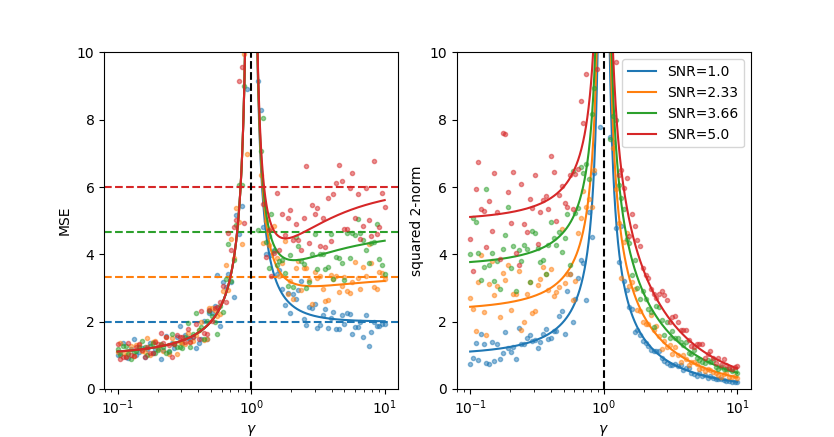
\includegraphics[width=1\linewidth, angle=0]{Figure_1} %11.4 cm wide
  \caption{Empirical (dots) and asymptotics (lines) for four different
    combinations of SNR, when $\gamma=n/p$. The dashed line at
    $\gamma=1$ indicates the interpolation point. (left) MSE on test
    set. The dashed lines is the MSE when $\gamma \rightarrow
    \infty$. (right) $||\theta||_2^2$.}
  \label{fig:double}
\end{figure}

\bibliographystyle{plain}
\bibliography{report2}

\end{document}
